%\part{Konstruktion}
%\chapter{Programmlogik}
%\section{QueryResolution}

\subsection{QuerySend}

\begin{figure}[htb]
  	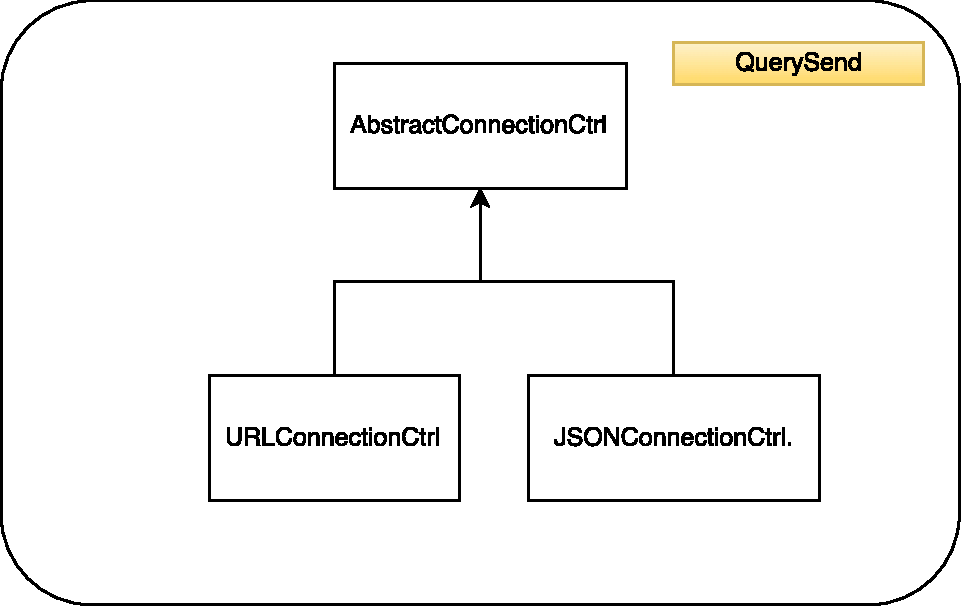
\includegraphics[width=\textwidth]{qr_querysend}
  	\caption{Aufbau des Moduls QuerySend}
	\label{fig:Aufbau des Moduls QuerySend}
\end{figure}

Im Modul QuerySend befinden sich die ConnectionController, welche für das Versenden der Anfrage zuständig sind. Die ConnectionController werden mithilfe von QueryBuild konfiguriert und erhalten den Parser (ResponseParse).

Bevor die Antwort an den TaskController weitergereicht wird, wird diese noch durch den Parser von NSData zu SearchResult umgewandelt.

\subsubsection{AbstractConnectionCtrl}
\subsubsection{JsonConnectionCtrl}
\subsubsection{URLConnectionCtrl}

%\paragraph{Paragraph}
%\subparagraph{Unterparagraph}
